\section{Introduction}

For this project, I wrote a simulation of an experiment and the code for analysis of the generated data, controlled by a GUI. The experiment concerns the (second order) 
statistics of a time independent speckle field , i.e. its spatial coherence. The statistical properties of the field can be controlled by a spatial filtering, 
and can be measured by interferometry, thus verifying the inverse proportionality relation between the width of the spatial spectrum and the correlation 
length predicted by the Wiener-Khintchine theorem. \\

In this document I will focus on the physics of the experiment, the main results obtained from the simulation and their interpretation, while I will review the 
characteristics of the code in a separated jupyter notebook.

\subsection{Set-up}

The arrangement of optical components in the main part of the experiment is as follows.

\begin{figure}[!ht]
    \centering
    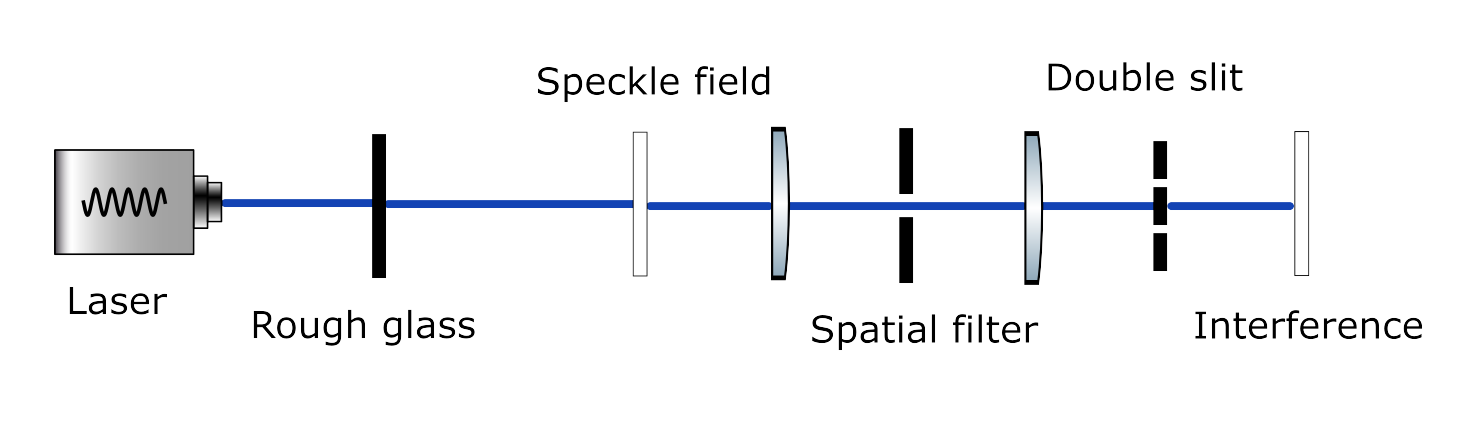
\includegraphics[width = .9\textwidth]{Img/setup.png}
    \caption{Set-up}
\end{figure}

The laser beam is assumed to have been expanded, filtered and collimated previously. The speckle field is produced by a rough glass surface, and is subsequently 
spatially filtered by a $4f$ set-up with a rectangular slit. Before filtering, the field already has a nonzero correlation length $\delta$ given by the Van Cittert-Zernike 
relation $\delta = z\lambda / D$ (where $z$ is the longitudinal propagation distance, $\lambda$ the wavelength and $D$ the diameter of the source, i.e. the collimated 
beam), which however is assumed to be negligible in comparison with the correlation induced by the filtering. \\

After filtering, the field has a (field) correlation function which is given by the Fourier transform of the filtered spectrum (Wiener-Khintchine theorem), 
which is

\begin{equation} \label{rect-corr}
    \gamma(s) = \mathrm{sinc}\,\left( \frac{\pi bs}{\lambda f} \right)
\end{equation}

for a rectangular filtering slit of width $b$ (here $f$ is the focal length of the lenses used for the filter). \\

This correlation function can be measured by Young interferometry: if the filtered field is probed by a double slit with separation $s$, one has the relation 

\begin{equation}
    \mathcal V = |\gamma(s)|,
\end{equation}

where $\mathcal V$ is the visibility, or contrast, of the interference pattern (the pattern is supposed to be averaged over an ensemble of speckle fields 
in order to capture the statistics). Once obtained the absolute value of $\gamma(s)$, the phase (which is always a $\pm 1$) can be inferred by the form of the 
pattern: if it has a central maximum, the phase is $+1$ (i.e., the two slits are on average in phase), while if it has a central minimum the phase is $-1$ 
(the two slits are out of phase). \\

By measuring the correlation function for different filtering widths one obtains the relation between correlation length and spectrum width.

\subsection{Simulation}

For simplicity, the simulation is done with $1$D instead of $2$D fields. The simulation also easily allows to filter the speckle field spectrum not only with 
a rectangular shape but e.g. with a gaussian shape, and it therefore showcases directly the Fourier transform relation given by the Wiener-Khintchine theorem. \\

Otherwise, the simulation closely follows the outline traced above: in the first part, a certain number ($\approx 200$) of $1$D speckle fields is generated 
and stored as csv files; in a second part, the  files are read and each one is fast-Fourier transformed, filtered, transformed back and used to generate an 
interference pattern. The patterns are then averaged over the ensemble, and the resulting averaged pattern is again stored as a csv. Finally, the patterns can 
be read and analyzed. \\